\documentclass[11pt]{scrartcl} % Font size
%%%%%%%%%%%%%%%%%%%%%%%%%%%%%%%%%%%%%%%%%
% Wenneker Assignment
% Structure Specification File
% Version 2.0 (12/1/2019)
%
% This template originates from:
% http://www.LaTeXTemplates.com
%
% Authors:
% Vel (vel@LaTeXTemplates.com)
% Frits Wenneker
%
% License:
% CC BY-NC-SA 3.0 (http://creativecommons.org/licenses/by-nc-sa/3.0/)
%
%%%%%%%%%%%%%%%%%%%%%%%%%%%%%%%%%%%%%%%%%

%----------------------------------------------------------------------------------------
%	PACKAGES AND OTHER DOCUMENT CONFIGURATIONS
%----------------------------------------------------------------------------------------

\usepackage{amsmath, amsfonts, amsthm} % Math packages
\usepackage{hyperref}
\usepackage{comment}
\usepackage{amsmath}
\usepackage{bbm}
\usepackage{algpseudocode, algorithm, algorithmicx}
\usepackage[toc,page]{appendix}
\usepackage[user,titleref]{zref}

\hypersetup{
   colorlinks=true,
   citecolor=red,
   linkcolor=cyan,
   filecolor=magenta,
   urlcolor=blue,
 }

\usepackage{url}
\usepackage{listings} % Code listings, with syntax highlighting

\usepackage[english]{babel} % English language hyphenation

\usepackage{graphicx} % Required for inserting images
\graphicspath{{Figures/}{./}} % Specifies where to look for included images (trailing slash required)

\usepackage{booktabs} % Required for better horizontal rules in tables

\numberwithin{equation}{section} % Number equations within sections (i.e. 1.1, 1.2, 2.1, 2.2 instead of 1, 2, 3, 4)
\numberwithin{figure}{section} % Number figures within sections (i.e. 1.1, 1.2, 2.1, 2.2 instead of 1, 2, 3, 4)
\numberwithin{table}{section} % Number tables within sections (i.e. 1.1, 1.2, 2.1, 2.2 instead of 1, 2, 3, 4)

\setlength\parindent{0pt} % Removes all indentation from paragraphs

\usepackage{enumitem} % Required for list customisation
\setlist{noitemsep} % No spacing between list items

%----------------------------------------------------------------------------------------
%	DOCUMENT MARGINS
%----------------------------------------------------------------------------------------

\usepackage{geometry} % Required for adjusting page dimensions and margins

\geometry{
	paper=a4paper, % Paper size, change to letterpaper for US letter size
	top=2.5cm, % Top margin
	bottom=3cm, % Bottom margin
	left=3cm, % Left margin
	right=3cm, % Right margin
	headheight=0.75cm, % Header height
	footskip=1.5cm, % Space from the bottom margin to the baseline of the footer
	headsep=0.75cm, % Space from the top margin to the baseline of the header
	%showframe, % Uncomment to show how the type block is set on the page
}

%----------------------------------------------------------------------------------------
%	FONTS
%----------------------------------------------------------------------------------------

\usepackage[utf8]{inputenc} % Required for inputting international characters
\usepackage[T1]{fontenc} % Use 8-bit encoding

% \usepackage{fourier} % Use the Adobe Utopia font for the document

%----------------------------------------------------------------------------------------
%	SECTION TITLES
%----------------------------------------------------------------------------------------

\usepackage{sectsty} % Allows customising section commands

\sectionfont{\vspace{6pt}\centering\normalfont\scshape} % \section{} styling
\subsectionfont{\normalfont\bfseries} % \subsection{} styling
\subsubsectionfont{\normalfont\bfseries} % \subsubsection{} styling
\paragraphfont{\normalfont\scshape} % \paragraph{} styling

%----------------------------------------------------------------------------------------
%	HEADERS AND FOOTERS
%----------------------------------------------------------------------------------------

\usepackage{scrlayer-scrpage} % Required for customising headers and footers

\ohead*{} % Right header
\ihead*{} % Left header
\chead*{} % Centre header

\ofoot*{} % Right footer
\ifoot*{} % Left footer
\cfoot*{\pagemark} % Centre footer

%-----------------------------------------------------------
%  Define new commands
%-----------------------------------------------------------
\DeclareMathOperator*{\argmax}{arg\,max}
\DeclareMathOperator*{\argmin}{arg\,min}
\DeclareMathOperator\supp{supp}

\newcommand*\Let[2]{\State #1 $\gets$ #2}

\DeclareMathOperator*{\E}{\mathbbm{E}}
\DeclareMathOperator*{\Z}{\mathbbm{Z}}
\DeclareMathOperator*{\R}{\mathbbm{R}} % Include the file specifying the document structure and custom commands

%----------------------------------------------------------------------------------------
%	TITLE SECTION
%----------------------------------------------------------------------------------------

\title{
	\normalfont\normalsize
	\textsc{Harvard Privacy Tools Project}\\ % Your university, school and/or department name(s)
	\vspace{25pt} % Whitespace
	\rule{\linewidth}{0.5pt}\\ % Thin top horizontal rule
	\vspace{20pt} % Whitespace
	{\huge Geometric Mechanism Notes}\\ % The assignment title
	\vspace{12pt} % Whitespace
	\rule{\linewidth}{2pt}\\ % Thick bottom horizontal rule
	\vspace{12pt} % Whitespace
}

\author{\LARGE Christian Covington} % Your name

\date{\normalsize\today} % Today's date (\today) or a custom date

\begin{document}

\maketitle

\section{Overview}
This document is a write-up of extra notes regarding implementations of the Geometric mechanism
in yarrow.

\section{Simple Geometric Mechanism}
\subsection{Background}
The \emph{Simple Geometric Mechanism} is an implementation of the Geometric
mechanism proposed in \cite{GRS12}. For a counting query $f$ with true value $f(d)$
and parameter value $\alpha \in (0,1)$, the $\alpha-$geometric mechanism outputs
$f(d) + \Delta$, where $\supp \Delta = \Z$ and
\begin{equation}
    \label{eq:grs12_geom}
    \Pr(\Delta = \delta) = \frac{1-\alpha}{1+\alpha} \alpha^{| \delta |}.
\end{equation}
This mechanism respects pure differential privacy, with a privacy loss parameter of $\alpha$.
To accommodate privacy parameters outside of $(0,1)$, we can choose a privacy parameter
$\epsilon > 0$ and let $\alpha = e^{-\epsilon}$. \newline

\subsection{Approximate Implementation}
Below is pseudocode that is pretty close to our implementation of the mechanism (more on the finer points later).
This directly matches the $\alpha$-Geometric mechanism from \cite{GRS12}.

\begin{algorithm}[H]
    \caption{(Almost) Simple Geometric Mechanism $M_{SG}(f(D), \epsilon)$}
    \label{alg:simp_geo_mec}
    \begin{algorithmic}[1]
        \State Let $f(D)$ be the count query we wish to privatize, $\epsilon$ be our privacy parameter and $\alpha = e^{-\epsilon}$.
        \State $u \gets$ Unif$(0,1)$
        \If{$u < \frac{1-\alpha}{1+\alpha}$} \label{alg_step:return_zero}
            \State return $f(D)$
        \Else
            \State $s \gets$ uniformly random draw from $\{-1, 1\}$ \label{alg:unif_draw}
            \State $g \gets$ Geom$(1 - \alpha)$ where $g \in \{1,2,\hdots\}$ \label{alg:draw_geom}
            \State return $f(D) + s \cdot g$
        \EndIf
	\end{algorithmic}
\end{algorithm}

\subsubsection{Proof that Algorithm \ref{alg:simp_geo_mec} is equivalent to Equation \eqref{eq:grs12_geom}}
First, note from Equation \eqref{eq:grs12_geom} that the mechanism returns $f(d)$ when $\Delta=0$,
which happens with probability $\frac{1-\alpha}{1+\alpha}$.
This is reflected in line \ref{alg_step:return_zero} of Algorithm \ref{alg:simp_geo_mec}. \newline

Now, we have handled the case where $\Delta = 0$, so let's manipulate Equation \eqref{eq:grs12_geom} a bit more.
For arbitrary $\delta \in \Z \setminus \{0\}$:
\begin{align*}
    \Pr(\Delta = \delta \vert \Delta \neq 0) &= \left( \frac{1}{1 - \Pr(\Delta = 0)} \right) \cdot \left( \frac{1-\alpha}{1+\alpha} \alpha^{| \delta |} \right) \\
               &= \left( \frac{1}{1 - \frac{1-\alpha}{1+\alpha}} \right) \cdot \left( \frac{1-\alpha}{1+\alpha} \alpha^{| \delta |} \right) \\
               &= \left( \frac{1 + \alpha}{2\alpha} \right) \cdot \left( \frac{1-\alpha}{1+\alpha} \alpha^{| \delta |} \right) \\
               &= \frac{1-\alpha}{2\alpha} \alpha^{|\delta|}.
\end{align*}
We know that the noise induced by the geometric mechanism should be symmetric, so let's now
consider only $\delta \in \Z^{+}$, with the knowledge that $\Pr(\Delta=\delta) = \Pr(\Delta=-\delta)$. This allows us
to remove the factor of 2 from the denominator and remove the absolute value around $n$:
\begin{align*}
    \Pr(\Delta = \delta | \Delta \neq 0) &= \frac{1-\alpha}{\alpha} \alpha^{\delta} \\
               &= \alpha^{\delta-1} \cdot (1-\alpha) \\
               &= (1-p)^{\delta-1} p \text{ [for $p = (1 - \alpha)$]}.
\end{align*}
Notice that this last statement is exactly the PDF of a Geom$(p)$ defined on $\{1,2,\hdots\}$ where
$p = 1-\alpha$. Thus, the combination of lines \ref{alg:unif_draw} and \ref{alg:draw_geom} from
Algorithm \ref{alg:simp_geo_mec} is sufficient to generate the modified distribution from
Equation \eqref{eq:grs12_geom} where we condition on $\Delta \neq 0$.

\subsection{Actual Implementation}
To this point, we have assumed that the noise generated from our mechanism has support
$\Z$ (we will call this the untruncated mechanism). This presents two major problems. \newline

First, recall that we need to sample from a Geometric distribution within our mechanism.
We do not want to use inverse transform sampling to do this, as doing so requires manipulation
of floating-point numbers that can lead to privacy violations.\footnote{See \cite{Mir12} and
\cite{Ilv19} for examples. \cite{BV17} is the only place I have seen the known problems
with floating-point numbers extended to their effects on inverse transform sampling.}
Therefore, we induce a Geometric distribution by randomly sampling bits until we
see a 1. If the distribution from which we are sampling has support $\Z$, we could hypothetically
sample an arbitrarily large number of flips and not see a 1. We would like some kind of guarantee
on the number of samples we need. \newline

Perhaps more importantly, the untruncated mechanism will sometimes yield nonsensical answers.
For a data set with known sample size $n$, the only reasonable answers to a counting query
are $\mathcal{S} = \{0,1,2,\hdots,n\}$. \newline

If the untruncated mechanism were to return a value
outside of $\mathcal{S}$, then we can clip the value so that it is back in the set.
This does not violate our privacy guarantee, as it is considered data-independent post-processing, and
can only help us in terms of absolute error. We will refer to this as the
\emph{Truncated Geometric Mechanism}, as introduced in \cite{GRS12}.
We also consider what truncating the eventual mechanism output means for how we need
to sample from the Geometric distribution. \newline

Let's return to Algorithm \ref{alg:simp_geo_mec}, but include truncation so that it
actually reflects the algorithm in yarrow. \newline

\begin{algorithm}[H]
    \caption{Simple Geometric Mechanism $M_{SG}(f(D), \epsilon, \text{ count\_min, count\_max, EFC})$}
    \label{alg:real_simp_geo_mec}
    \begin{algorithmic}[1]
        \State Let $f(D)$ be the count query we wish to privatize, $\epsilon$ be our privacy parameter, count\_min be the minimum
        possible count (likely 0), count\_max be the maximum possible count (probably $n$), and EFC (enforce\_constant\_time) be a boolean
        for whether or not we want to enforce our geometric sampling to always take the same number of steps.
        \State Let $\alpha = e^{-\epsilon}$.
        \State $u \gets$ Unif$(0,1)$
        \If{$u < \frac{1-\alpha}{1+\alpha}$}
            \State return $f(D)$
        \Else
            \State $s \gets$ uniformly random draw from $\{-1, 1\}$
            \State $g \gets$ $\text{Geom}_{Trunc}(1 - \alpha)$ where $g \in \{1,2,\hdots, \text{count\_max} - \text{count\_min}\}$
            \State return $\text{max}\bigg( \text{count\_min}, \text{min}\big(f(D) + s \cdot g, \text{count\_max}\big) \bigg)$ \label{alg:clipped_output}
        \EndIf
	\end{algorithmic}
\end{algorithm}
You can see in line \ref{alg:clipped_output} of Algorithm \ref{alg:real_simp_geo_mec} where we clip the final output
to the set
\[ \mathcal{S} = \{\text{count\_min}, \text{count\_min} + 1, \hdots, \text{count\_max}\}, \]
again keeping in mind that, in general, count\_min and count\_max will be $0$ and $n$, respectively. \newline

Our final step is to define Geom$_{Trunc}$. We know that our raw count $f(D)$ must be between count\_min and count\_max
and that our mechanism will eventually return a result between those same bounds. Therefore, the absolute maximum noise
we could ever add is $r = \text{count\_max} - \text{count\_min}$; any more would always put us outside of the set $\mathcal{S}$
and eventually be clipped back into the set. Therefore, we can sample at most $r$ bits when generating the draw
from the Geometric distribution. If we have sampled $r$ bits and not seen a 1, then we can set $g = r$ without
affecting our eventual result.

\subsection{More notes on truncation}
We noted above that truncation can only help our accuracy (in terms of $\ell_1$ error), but it is very possible that our accuracy
remains poor even after truncation. Imagine that we have data $D$ with $n=30$ and want to release a counting query on
some predicate $\phi$ for which
\[ \phi(D) = \left( \sum_{i=1}^{n}\mathbbm{1} [\phi(d_i) = 1] \right) = 20, \]
where the $d_i$ are the elements of $D$. If we wanted to release a differentially private version of $\phi(D)$, we
could use the Geometric mechanism. The distribution of answers we would get for the mechanism, with a privacy parameter of $\epsilon = 0.1$
are shown in orange below.\footnote{We will come back to why we plotted results for $\phi(D) = 19, 20,$ and $21$.}

\begin{figure}[h]
    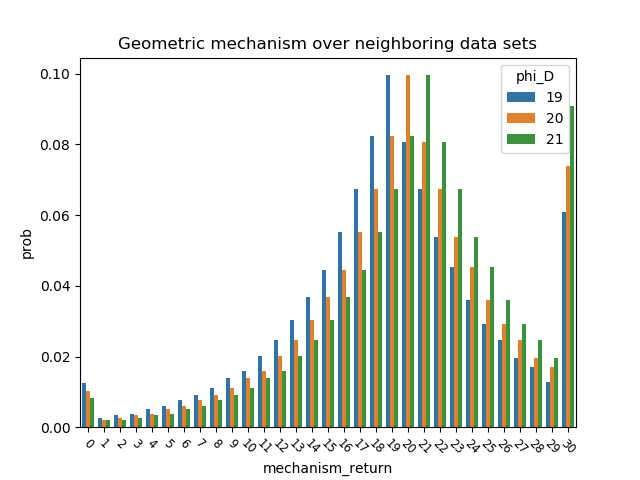
\includegraphics[width = \textwidth]{truncated_geometric_mech_dist.png}
    \caption{Truncated Geometric Mechanism Output}
\end{figure}
With this strategy, we are getting as bad an answer as possible (0) with probability $\approx 0.075$ and are
getting answers at the extreme ends of our support (0 and 30) with probability $\approx 0.25$.
We would like to see if there is a way to maintain the DP properties of our mechanism, while also
concentrating more of the mass of this distribution around ``good answers''. \newline

One seemingly reasonably way to do this would be to simply ignore any events that produce truncated noise,
that is if our generated noise $\Delta$ is either less than $-\phi(D)$ or greater than $n - \phi(D)$.
We see that
\begin{align*}
    \Pr\left(\Delta < -\phi(D)\right) &= \frac{\alpha^{\phi(D) + 1}}{1 + \alpha} \\
    \Pr\left(\Delta > n - \phi(D)\right) &= \frac{\alpha^{n - \phi(D) + 1}}{1 + \alpha}
\end{align*}
Let $T_D$ be the event that our mechanism produces noise that must be truncated. Then,
\[ \Pr(T_D) = \Pr\left(\Delta < -\phi(D)\right) + \Pr\left(\Delta > n - \phi(D)\right) = \frac{\alpha^{\phi(D)+1} + \alpha^{n-\phi(D)+1}}{1+\alpha} \]
We could think about creating a noise distribution in which we never produce noise that needs to be truncated, and
the probability that we produce any allowable amount of noise is increased by a factor of $\frac{1}{1 - \Pr(T_D)}$.
This leads to a problem though; $\Pr(T_D)$ is a function of our data, and thus the multiplicative scaling factor
will differ between neighboring data sets. For pure DP, we need the probability of all outcomes on neighboring data sets to be bounded
by $e^{\epsilon}$; we know that the regular geometric mechanism satisfies this, but if we are scaling probabilities
on neighboring data sets by different factors, we can no longer be sure that the bound holds.
We would like to be able to reason about the extent to which these different scaling factors could affect our
privacy guarantee. We will attempt to do so by considering the maximum extent to which the scaling factors differ
for given values of $\alpha$ and $n$. Note that we need to remove the dependence on $\phi(D)$ in order to retain our DP guarantee. \newline

Let $D', D''$ be data sets that neighbor $D$ such that $f(D') + 1 = f(D) = f(D'') - 1$. Then we have
\begin{align*}
    \Pr(T_{D'}) &= \frac{\alpha^{\phi(D) + 2} + \alpha^{n-\phi(D)}}{1+\alpha} \\
    \Pr(T_{D''}) &= \frac{\alpha^{\phi(D)} + \alpha^{n-\phi(D)+2}}{1+\alpha}.
\end{align*}
Let's now consider the the quantities
\begin{align}
    \label{eq:L_U}
    L_{\phi(D)} &= \frac{\Pr(T_D)}{\Pr(T_{D'})} = \frac{\alpha^{2 \phi(D) + 1} + \alpha^{n+1}}{\alpha^{2 \phi(D) + 2} + \alpha^{n}} \\
    U_{\phi(D)} &= \frac{\Pr(T_D)}{\Pr(T_{D''})} = \frac{\alpha^{2 \phi(D)+1} + \alpha^{n+1}}{\alpha^{2 \phi(D)} + \alpha^{n+2}}. \nonumber
\end{align}
We cannot use these quantities directly, as they will leak extra information about our data.
However, if we can get global upper and lower bounds on both $L$ and $U$,
then we will have bounds on the extent to which $\Pr(T)$ can differ on arbitrary neighboring data sets.
Let's start by looking at the partial derivatives of $L,U$ with respect to $\phi(D)$,
\begin{align*}
    \frac{\partial L_{\phi(D)}}{\partial \phi(D)} &= -\frac{2(\alpha^2-1) \cdot \ln(\alpha) \cdot \alpha^{2\phi(D)+n+1}}{(\alpha^{2\phi(D)+2}+\alpha^{n})^2} < 0 \\
    \frac{\partial U_{\phi(D)}}{\partial \phi(D)} &= \frac{2(\alpha^2-1) \cdot \ln(\alpha) \cdot \alpha^{2\phi(D)+n+1}}{(\alpha^{2\phi(D)}+\alpha^{n+2})^2} > 0.
\end{align*}
We know the sign of each of those because $\alpha \in (0,1)$ implies that the numerator is positive, and the denominator is
always positive because it is a quantity squared. Therefore, we know that both $L_{\phi(D)}$ and $U$ are monotonic in $\phi(D)$,
so we can just consider the values of $L_{\phi(D)}$ and $U_{\phi(D)}$ for our most extreme values, where $\phi(D) \in \{0, n\}$.
We know then that, for all $n > 0$:
\begin{align*}
    L_{n} = \frac{\alpha^{2n+1} + \alpha^{n+1}}{\alpha^{2n+2} + \alpha^n} \leq \hspace{2pt} &L_{\phi(D)} \leq \frac{\alpha^3 + \alpha^{n+1}}{\alpha^4 + \alpha^n} = L_{1} \\
    U_{0} = \frac{\alpha + \alpha^{n+1}}{1 + \alpha^{n+2}} \leq \hspace{2pt} &U_{\phi(D)} \leq \frac{\alpha^{2n-1} + \alpha^{n+1}}{\alpha^{2n-2} + \alpha^{n+2}} = U_{n-1}.
\end{align*}
Note that we do not define $L_0$ or $U_n$ because if $D$ is such that $\phi(D) = 0$ or $\phi(D) = n$, there are no
data sets that produce a smaller (or larger) count, respectively. \newline

Because $L_n, U_0 < 1 < L_1, U_{n-1}$ and we want the maximum overall difference in our scaling factor, it is sufficient to find
\[ M = \max \left( \frac{1}{L_n}, \frac{1}{U_0}, L_1, U_{n-1} \right). \]
Each of these is a function only of $\alpha$ and $n$, where $\alpha = e^{-\epsilon}$, so we can calculate $M$
from only our privacy loss parameter and sample size. So, if the probabilities outputs on neighboring data sets
were bounded by $e^{\epsilon}$ for the regular geometric, they are now bounded by $M \cdot e^{\epsilon}$.
Noting that $M \cdot e^{\epsilon} = e^{\ln(M) + \epsilon}$, we see that if we use $\epsilon$ as our
privacy loss parameter, we end up getting a guarantee as if we asked for $e^{\ln(M) + \epsilon}$.
Likewise, if we truly want an $\epsilon$ guarantee, we could parameterize the geometric with
$\epsilon' = \epsilon - \ln(M)$. \newline

One plausible way to use this is to parameterize the \emph{Truncated Geometric Mechanism}
with $\epsilon'$ rather than $\epsilon$ and simply reject any mechanism return value that is outside
of our range of feasible counts.
In my testing, this method ended up being pretty low-utility, inducing a nearly uniform distribution
of outputs over the set of possible counts.
\begin{figure}[H]
    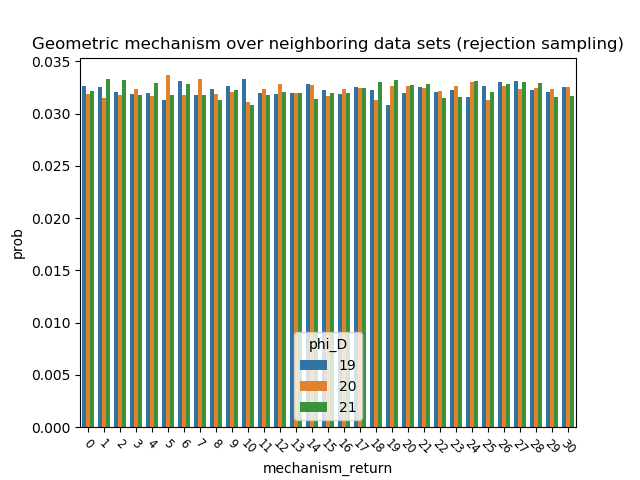
\includegraphics[width = \textwidth]{rejection_sampling_geometric_mech_dist.png}
    \caption{Truncated Geometric Mechanism Output with Rejection Sampling}
\end{figure}

The problem appears to be with $\epsilon'$ --
for small $\epsilon$, the additive change by $\ln(M)$ is, multiplicatively, quite large,
and the noise we need to add increases dramatically. For large $\epsilon$, we typically do not
need to worry about pushing mass toward the center of the distribution, as it is already there. \newline

One area I thought we might be able to improve was in the calculation of $M$.
Earlier, we made a worst-case assumption about our data set $D$ in order to remove the
dependence of $M$ on $D$. One could imagine, however, releasing a DP version of some function on $D$
and having $M$ have a dependence on that function. I tried releasing a DP estimate of
$\phi(D)$, which we call $\hat{\phi(D)}$ using the Exponential mechanism and using that estimate as input for
$L,U$ from Equation~\ref{eq:L_U}. However, because we are not actually using $\phi(D)$,
the calculation of $M$ based on $\hat{\phi(D)}$ may not actually be an upper bound on the
difference in the scaling factor for our real data. \newline

This is a problem I do not know how to solve.
We cannot restrict the feasible set for the Exponential mechanism to values of $\hat{\phi(D)}$
for which the associated $M$ is an actual upper bound on the actual scaling factor because the choice of feasible
set must be independent of the data. I considered creating a score function for the Exponential mechanism
that greatly penalizes values of $\hat{\phi(D)}$ for which $M$ is not an upper bound on the
actual scaling factor, but this makes the sensitivity of the score function very difficult to reason about
without just assuming a trivial worst-case.

\bibliographystyle{alpha}
\bibliography{geometric}
\end{document}